\chapter{外文资料的调研阅读报告或书面翻译}
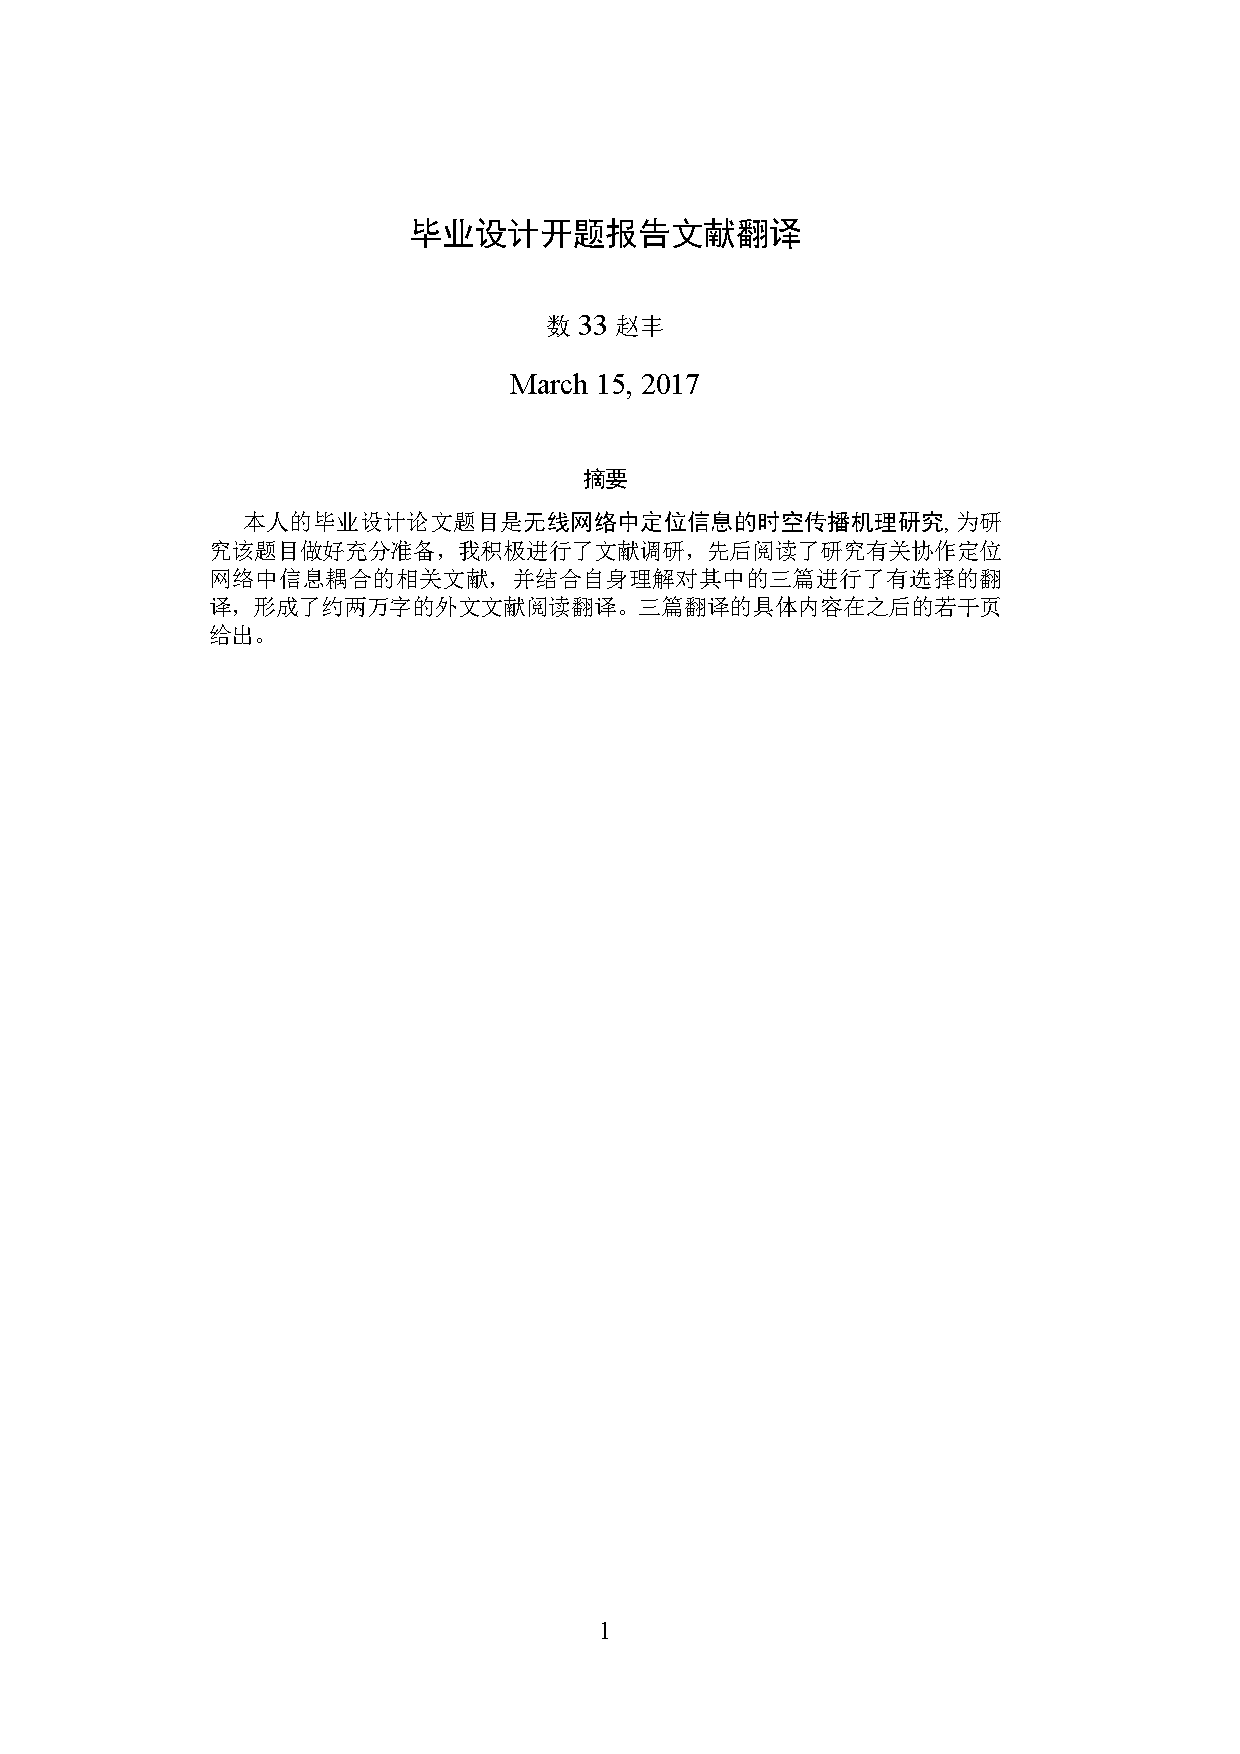
\includepdf[pages=-]{translation.pdf}
\chapter{公式的推导}
\section{建模过程的一些推导过程}
\subsection{定位问题中费舍尔信息矩阵一般结构推导}\label{A_F_1}
在非协作单节点定位中,测量量的联合概率分布由式(\ref{eq:single})给出,费舍尔信息矩阵是费舍尔信息量的自然推广,在满足一定正则性的条件下,费舍尔信息矩阵可以写成:
\begin{equation}
I(\bm{p})=-\mathbb{E}_{\bm{x}}(\bigtriangledown_{\bm{p}} \log f(\vec{x}|\bm{p}))^T(\bigtriangledown_{\bm{p}} \log f(\vec{x}|\bm{p}))
\end{equation}
其中f是随机向量$\vec{x}$的密度函数,利用上面的公式,首先对式(\ref{eq:single})取对数并求梯度得:
\begin{equation}
\bigtriangledown_{\bm{p}}\ln f=-\sum_{i=1}^{N_b}\frac{||\bm{p}_i^b-\bm{p}||-x_i}{\sigma_i^2}\frac{\bm{p}^b_i-\bm{p}}{||\bm{p}^b_i-\bm{p}||}
\end{equation}
注意到$\frac{||\bm{p}_i^b-\bm{p}||-x_i}{\sigma_i}~ N(0,1)$,所以按照费舍尔信息矩阵的定义可得到式(\ref{eq:uu})的结果。
\section{研究成果的一些推导过程}
\subsection{单节点动态定位问题等效费舍尔信息矩阵推导}\label{B_F_1}
为简化符号,记$\bm{u}:=\bm{u}_{12}$,2阶单位阵记为$\bm{I}_2$,由等效费舍尔信息矩阵的定义,有
\begin{equation}
  T_1=\lambda \bm{I}_2+\bm{u}\bm{u}^T-\bm{u}\bm{u}^T K_2^{-1}\bm{u}\bm{u}^T
  =\lambda \bm{I}_2+(1-\bm{u}^T K_2^{-1}\bm{u})\bm{u}\bm{u}^T
\end{equation}
因为$\bm{u}\bm{u}^T=U\begin{pmatrix}
                     1 & 0 \\
                     0 & 0
                   \end{pmatrix}U^{-1}$,其中$U$是由$\bm{u}$的方向角确定的二维旋转矩阵,所以
$T_1$相似于$\begin{pmatrix}
                           \lambda+1-\bm{u}^T K_2^{-1}\bm{u} & 0 \\
                           0 & \lambda
                         \end{pmatrix}$
下面化简$1-\bm{u}^T K_2^{-1}\bm{u}$注意到$K_2=\bm{u}\bm{u}^T+J_2$,$J_2$是不考虑前(i-1)个时刻节点位置写出的等效费舍尔信息矩阵,所以
\[
1-\bm{u}^T (\bm{u}\bm{u}^T+J_2)^{-1}\bm{u}
\]
由式(\ref{eq:woodbury})可得
\begin{equation}
1-\bm{u}^T (\bm{u}\bm{u}^T+J_2)^{-1}\bm{u}
=(1+\bm{u}^T J_2^{-1}\bm{u})^{-1}
\end{equation}
进一步设$v:=\bm{u}_{23}$,则$J_2=\lambda \bm{I}_2+(1-\bm{v}^T K_3^{-1}\bm{v})\bm{v}\bm{v}^T=V\begin{pmatrix}
                     \lambda+1-\bm{v}^T K_3^{-1}\bm{v} & 0 \\
                     0 & \lambda
                   \end{pmatrix}V^{-1}$
设$\bm{u}=(\cos\theta,\sin\theta)^T,\bm{v}=(\cos\phi,\sin\phi)^T$,则
\[
V^{-1}\bm{u}=\begin{pmatrix}
                     \cos\phi & \sin\phi \\
                     -\sin\phi & \cos\phi
                   \end{pmatrix}\binom{\cos\theta}{\sin\theta}=\binom{\cos(\theta-\phi)}{\sin(\theta-\phi)}=:w
\]
所以
\[
1-\bm{u}^T (\bm{u}\bm{u}^T+J_2)^{-1}\bm{u}=(1+\bm{w}^T \begin{pmatrix}
                     \lambda+1-\bm{v}^T K_3^{-1}\bm{v} & 0 \\
                     0 & \lambda
                   \end{pmatrix}^{-1}\bm{w})^{-1}
                   =\frac{1}{1+\frac{\cos^2(\theta-\phi)}{T_2}+\frac{\sin^2(\theta-\phi)}{\lambda}}
\]
递推可得一般形式:
终止条件:当计算到原费舍尔信息矩阵的右下角时$T_{N_a-1}=\lambda$,
所以对$N_a$维矩阵,协作方向有$N_a-1$,而得到的有限连分式数列也恰有$N_a-1$项。
\subsection{单节点动态定位问题等效费舍尔信息衰减上下界}\label{B_F_2}
考虑在原有基础上增加一层节点,即利用上距离时间中点前后更远的两个时刻的位置,由对称性我们只需考虑单边,
于是协作层数由原来的$N_a-1$变为$N_a$,等效费舍尔信息矩阵较大的特征值分别记为$T_1,T'_1$,为便于比较,我们在$T_1$中引入虚拟节点将其层数也拓展为$N_a$,它只有锚点的定位信息,这样它们的区别是连分式的末端$T_{N_a+1}=\lambda$,$T'_{N_a+1}=\lambda+\frac{1}{1+1/\lambda}$
对$|T_1-T'_1|$从外向里通分得:
\[
|T_1-T'_1|=\frac{\cos^2\theta_1|\frac{1}{T_2}-\frac{1}{T'_2}|}{(1+\frac{\sin\theta_1}{\lambda}+\frac{\cos\theta_1}{T_2})
(1+\frac{\sin\theta_1}{\lambda}+\frac{\cos\theta_1}{T'_2})}\leq |\frac{1}{T_2}-\frac{1}{T'_2}|
\]
继续放缩$|\frac{1}{T_2}-\frac{1}{T'_2}|$有:
\[
|\frac{1}{T_2}-\frac{1}{T'_2}|= \frac{\cos^2\theta_2|\frac{1}{T_3}-\frac{1}{T'_3}|}{(1+\lambda(1+\frac{\sin\theta_2}{\lambda}+\frac{\cos\theta_2}{T_3}))
(1+\lambda(1+\frac{\sin\theta_2}{\lambda}+\frac{\cos\theta_2}{T'_3}))}\leq |\frac{1}{T_3}-\frac{1}{T'_3}|\frac{1}{(1+\lambda)^2}
\]
逐次递推得
\[
|T_1-T'_1|\leq \frac{1}{(1+\lambda)^{2(N_a-1)}} |\frac{1}{T_{N_a+1}}-\frac{1}{T'_{N_a+1}}|
\]
而:
\[
|\frac{1}{T_{N_a+1}}-\frac{1}{T'_{N_a+1}}|=\frac{1}{\lambda^2+2\lambda}
\]
另一方面,因为$T_2,T'_2\geq \lambda$
\[
|T_1-T'_1|\geq \frac{\cos^2\Delta\theta|\frac{1}{T_2}-\frac{1}{T'_2}|}{(1+1/\lambda)^2}
\]
\[
|\frac{1}{T_2}-\frac{1}{T'_2}|\geq \frac{\cos^2\Delta\theta|\frac{1}{T_3}-\frac{1}{T'_3}|}{(2+\lambda)^2}
\]
逐次递推得下界。
